\chapter{Virtual Private Overlays}
\label{vpo}
While Structured P2P overlays provide a scalable, resilient, and self-managing
platform for distributed applications, their adoption rate has been slow
outside data distribution services such as BitTorrent and eDonkey.  General use
of structured P2P systems, especially in applications targeting homes and
small/medium businesses (SMBs), has been limited in large part due to the
difficult nature of securing such systems to the level required by these users.
Applications in home and SMBs may need a greater level of trust than what can
be guaranteed by anonymous contributors in free-to-join overlays, but many these
users lack the resources or expertise necessary to bootstrap a private P2P
overlays particularly in constrained wide-area network environments where a
significant amount of or all peers may be behind Network Address Translation
devices (NAT).

There are many different P2P applications used in home and small business,
primarily for collaboration and sharing, including data storage, media sharing,
chat, and system maintenance and monitoring.  Applications that currently
provide these functionalities fall into two categories:  anonymous, fully
decentralized free-to-join P2P systems and distributed systems with P2P
communication that rely on a third party to provide discovery and management.
While using a third party service provides a desirable level of trust for many
users, it has significant drawbacks such as vendor lock-in, which may result in
lost data, down time, and scalability constraints.

An example of a useful small business application that falls into the latter
category is LogMeIn's~\cite{logmein} software products LogMeIn Pro and Hamachi.
LogMeIn Pro allows users to remotely manage and connect with their machines so
long as they are willing to use LogMeIn's software and infrastructure.  Hamachi
allows users to establish decentralized VPN links using centralized session
management.  Both applications assist in the remote maintenance and monitoring
of computers without requiring the user to implement the networking
infrastructure provided by LogMeIn.

Some examples of P2P applications for homes and small businesses in development
are P2PSIP~\cite{p2psip} and P2Pns~\cite{p2pns}.  P2PSIP enables users to
initiate, through decentralized means, visual and audio communication, while
P2Pns allows users to deploy a decentralized naming service.  Both applications
allow users to contribute and benefit from all members of the system without
the regulation of a third party, but lack the ability to allow users to
centrally secure and manage their own subset of the systems.

Distributed data store applications like Dynamo~\cite{dynamo} and
BigTable~\cite{bigtable} have the ability to store data using a completely
decentralized system.  Though these systems are highly scalable and fault
tolerant, the software uses an insecure overlay.  Therefore all instances
need to run in a secure environment, whether that is in a single institution
or across a largely distributed environment using a VPN.

This chapter reviews security issues and current examples of security in P2P.
Using the motivation of user centric and friendly systems, I present a method
for users to create their own secure, private overlays using the same core
overlay primitives as public overlays without the constraints imposed on them
by lacking dedicated, public resources through the use of a shared,
free-to-join public overlay.

\section{Security Issues in Structured Overlays}
While there has been much research~\cite{secure_routing} in securing overlays
through decentralized mechanisms that attempt to prevent collusion known as
a Sybil attack~\cite{sybil}, these mechanisms do not create private overlays.
One approach mentioned does provide a natural lead into such environments by
using of a pay-to-use service to mitigate the chances of an overlay attack,
whereby the pay to use service uses a CA to sign node IDs.  The work does not
describe how to efficiently implement such a system.  Other
projects~\cite{stone, tor} combine trusted overlays with anonymous members,
though it could be reasonably argued these services are not applicable to small
or medium business, which would prefer to have a private overlay.  None of the
works focus on how to apply such models to systems that are constrained in
network connectivity, e.g. by NATs.

\section{Secure Overlays}
\label{secure_overlays}
In recursive overlays, there are two forms of overlay communication:
\begin{itemize}
\item \textbf{Point-to-point (PtP)}:  Direct connections between peers in an
overlay, such as a UDP, TCP, or relay connecting two peers.  In an iterative
system, all messages are PtP.
\item \textbf{End-to-end (EtE)}:  Messages passed through an overlay from
peer to peer, used typically for application communication such as DHT queries.
\end{itemize}
Iterative overlays do not distinguish between the two forms of communication as
all communication is directly between two peers and never indirectly
communicated unless relays are used.

Securing communication in overlays using iterative routing without relays and
static IP addresses can easily be done using TLS~\cite{tls} or DTLS~\cite{dtls}
with certificates bound to the node's IP address.  Similarly PtP can be secured
in recursive overlays with static address.  Including relays, NAT traversal, or
EtE in recursive overlays complicates the issue.  NAT traversal cannot must
bind the certificate to something other than the peers IP address. Relays and
EtE routing require communicating through indirect communication and existing
security libraries are built on top of sockets and thus are not applicable in
these environments.  Furthermore, overlays are not reliable environments and
thus without a reliable overlay primitive TLS cannot be employed.  DTLS can
be applied because it supports lost and out of order messages, though the
implementation must support usage without a socket.  In this section, I discuss
how to bind security protocols and a certificate model to an overlay system
addressing the issue of applying DTLS to overlays and binding certificates to
individuals even in NAT environments.

The key to my approach is the abstraction used in the communication layer,
making EtE and PtP traffic appear identical. In this approach, all messages
are treated as datagrams, which are sent over abstracted senders and receivers
as filters illustrated in Figure~\ref{fig:senders_receivers}.  This allows use
of secure tunnels over these links with no application changes.

Exchanged certificates need a mechanism to verify authenticity.  Like an
Internet browser, this verification should happen automatically with no user
intervention.  Typically for SSL-derivatives, the certificates have the owner's
IP address or domain name as part of the certificate's common name field.  In
the prototype system, the certificate is bound to each individual node ID.
That way, a single certificate cannot be used for multiple peers in the
overlay, making it difficult for an adversary to launch Sybil attacks.

\subsection{Forming the Connection}
In overlay systems, a peer's connection manager requests an outgoing
connection to another peer in the system.  This triggers the creation of a
socket (UDP or TCP), which is wrapped in the abstracted sender and receiver
models.  The abstracted models arrive into the security handler, which
authenticates in both directions and creates a secure session.  The session is
wrapped in the same abstracted model and presented to the overlay system as a
direct connection to the remote peer.  To keep the system abstract, the security
model and the wrapped sockets know nothing about the overlay, and so the overlay
should verify the certificate to ensure identity.

Because EtE communication is application-specific, it requires a slightly
different path.  For that purpose, users are able to obtain a secure EtE
sender through an instance factory, allowing multiplexing of secure senders for
multiple applications as well as PtP communication.  Once an application
requests the sender, the module passes a sender / receiver model to the
security handler, like in the PtP process.  Once the security initialization
has completed, the resulting sender / receiver is verified automatically for
proper identity.  If that succeeds, messages sent using the EtE sender will
arrive at the remote party, decrypted and authenticated by the security
handler, and delivered to the overlay application, who will deliver to the
remote party's handler for such messages.  Since overlay applications will be
sending and receiving unencrypted as well as encrypted EtE traffic, the handler
must verify that the packet was sent from a secure end point.  This assumes
that an application using an overlay has already implemented verification of
node ID to some application mapping.  For example, an application could be
aware that node ID X maps to user Y, therefore if a secure message coming from
node ID Z says that it is user Y, an application should drop the packet.

\subsection{Datagram Constraints}
UDP is a connectionless protocol, enabling applications that use it to easily
become victims of denial of service attacks.  This is because packets sent to
the receiver can have a spoofed source address, unless the outgoing gateway
prevents this from occurring, egress filtering.  For each spoofed attempt, the
security system maintains state, which might eventually be overloaded.  In TCP,
this is hampered due to the three message handshake, which verifies that a
source address is not spoofed, prior to creating security state for the
connection.  To reduce the potential of these spoofing attacks prior to
establishing a secure connection, DTLS (like Photuris~\cite{photuris}) uses a
stateless cookie for each remote peer.  In DTLS, the cookie is usually based
upon the remote peer's IP and the current time.  In prototype model, which
deals with abstracted systems and IP addresses are likely to be NAT-translated,
this approach does not work.  Though for PtP, it is possible to use the address
and port from which the remote peer last sent a message from.  For EtE traffic,
the node ID can be used for cookie calculation.  Because we are building on
existing senders and receivers that already have state, we use the object's
memory pointer or hash value instead, though this leads us down a similar path
of denial of service found in TCP SYN attacks.

\subsection{Implementation}
To provide security, I investigated two approaches:  reusing OpenSSL's DTLS
implementation and a platform-independent approach similar to DTLS using C\#
and cryptography routines provided by .NET.  A constraint in the development is
that EtE communication must be able to be secured, which could be enabled by a
filter approach using memory buffers instead of sockets.

Implementation of an OpenSSL DTLS filter was non-trivial, as documentation is
sparse providing the possibility for varied approaches.  Traditionally, DTLS
uses the DGRAM (datagram) BIO (I/O abstraction) layer, which provides a reliable
UDP layer.  To support the filter behavior to support both EtE and PtP traffic,
one memory BIO was used for incoming traffic and another for outgoing traffic.
Memory BIOs provide pipes using RAM: data written to the BIO can then be read
in a first in, first out ordering.  Incoming messages written to or outgoing
messages read from the DTLS read or write BIOs, respectively, are either
encrypted data packets or handshake control messages.  Sending and receiving
clear text messages occur at the DTLS SSL object layer.  The pathway for
sending a clear text packet begins with the user performing an SSL\_write
operation, retrieving the encrypted data by performing a BIO\_read on the write
BIO, and sending the data over the network.  At the remote end, the packet is
passed to the SSL state machine by performing a BIO\_write on the incoming BIO
followed by a SSL\_read; the result will be the original clear text message.
This process also needs to handle control messages; we provide clear context in
Figure~\ref{fig:dtls_filter}.  As an aside, OpenSSL supports a SSL filter
BIO, though it will not work for this purpose as BIOs that are inserted are
expected to have two pipes, like a socket or two memory buffers.  Also the only
benefit of using the filter BIO would be that it manages auto-renegotiation,
which can be implemented in user code by monitoring time and received byte
count.  Other operations such as certificate verification and cookie generation
are handled by SSL callbacks, which hook into the security framework.

OpenSSL is a de-facto standard, with US federal government approved code (FIPS)
and platform portability, though during my development involving the platform I
experienced a few issues.  The portability provided by OpenSSL is limited to
API (Application Programming Interface) and not ABI (Application Binary
Interface), which requires a platform-specific library be either installed or
distributed with the application.  Whereas the purpose in using C\#, like Java,
is that a single binary can run on any platform.  To use unmanaged libraries
from a managed language requires a marshaling wrapper to handle the
translation; there is such a wrapper for OpenSSL~\cite{openssl.net}.  A
constraint we found when using the library was the naming of the OpenSSL
libraries was not consistent across platforms and, additionally, Windows lacked
a formal installation method.

In using the OpenSSL library with DTLS, in version 0.9.8k, renegotiation of
security parameters was broken resulting in deadlocked DTLS sessions.  Whereas
in 1.0.0-beta3 (the latest released beta) DTLS renegotiation worked, though often
crashing due to segmentation faults.  These issues were the motivation
for the creation of a platform independent security architecture similar to
DTLS written in C\#.  To provide for flexibility between the two approaches,
I created a security overlord that treats each approach like a filter.
Treating each implementation as a filter allows incoming control and data
messages to be pushed into the object and data and control messages to be
pulled out of the object.  While I believe OpenSSL's DTLS to be a superior
choice due to its prevalence and being well studied, it is non-trivial to make
available for all platforms.  Because my goal is to provide a safe yet easy to
use the overlay package, I leave the decision up to the user which protocol to
use.   I believe those interested in testing the system will start with the
.NET security stack and migrate to the OpenSSL DTLS stack.


% The handshake used is shown in Figure~\ref{fig:dtls}.
%\begin{figure}[h]
%\centering
%\includegraphics[width=2.75in]{in_progress.eps}
%\caption{DTLS Handshake}
%\label{fig:dtls}
%\end{figure}

Since symmetric keys work on limited block size, they use modes of operation
to encrypt or decrypt large sets of blocks.  Because DTLS uses an unreliable
transfer mechanism, each message should be able to be decrypted without the use
of previous messages.  As suggested in the DTLS paper, we used cipher-block
chaining (CBC) with a new initialization vector (IV) for each message.  During
analysis of the C\# implementation, it was apparent that generating an IV was
expensive but the initialization of an additional CBC state machine was even
more.  To reduce these costs, the sender always uses the same CBC state machine
and prepends the last cipher-block to the beginning of the next message.  Upon
reception, a receiver compares the prepended message to a cache of CBC state
machines stored by the current state, if there is a match, then the CBC state
machine can be used, otherwise, if the packet is received out of order the
receiver can start a new CBC state machine to decrypt the packet.  This issue
does not appear in the OpenSSL implementation of CBC.

\section{Private Overlays}
\label{private_overlays}
The main components involved in starting and maintaining a private overlay
are 1) dissemination of the security credentials and its name, 2) connecting
with and storing data in the public overlay, and 3) discovering and connecting
with peers in the private overlay.  Step 1) can be application-specific; we
propose a generic interface that is useful in many applications, through the
use of groups as described in Section Section~\ref{group_overlays}.  For 2),
we presume the usage of a structured overlay as described in
Chapter~\ref{structured_p2p}.  In this section, we discuss 3), the steps
involved in creating and connecting to a private overlay after the user has
obtained group information and has connected to a public overlay.

To connect with and create a private overlay, the application performs the
following steps%, as depicted in Figure~\ref{fig:private_overlay_states}:
1) connect to the public overlay; 2) store node ID in the public overlay's DHT
at the private group's key; 3) query the public overlay's DHT at the private
group's key; 4) start an instance of the private overlay with the well-known
end points being the node IDs retrieved from the DHT; and 5) upon forming a
link with a member in the private overlay, the node follows the standard
approach for linking to neighbors and shortcuts but using secure PtP links to
restrict connections to members of the private overlay.

While a node does not need to maintain membership in the public overlay once
connected with the private overlay, it will benefit the private overlay for it
to do so.  If the peer remains in the private overlay, other peers can discover
the node while following the same set of steps and, for NAT traversal purposes,
as discussed in the next paragraph.  Because the public overlay and its DHT
provides a means for discovery, nodes should maintain their node ID in the public
overlay's DHT.  If the DHT employs a lease or soft state system, while online
the node must renew the lease prior to expiring.

During the formation of the private overlay, peers may find that they are
unable to form direct connections with other members of the private overlay
even while using STUN based NAT traversal.   To address this problem, peers can
1) use TURN NAT traversal in the nodes overlay as in Chapter~\ref{structured_p2p}
or 2) use the public overlay as an extra routing massive TURN infrastructure.
The TURN NAT traversal technique has both peers connect with each other's near
neighbors in order to form a 2-hop connection with each other.  The 2-hop route
can either be enforced through a static route or through EtE greedy routing.
Due to the abstractions in the system, the public overlay can be treated as
another mechanism to create PtP links, thus while packets may use EtE routing
on the public overlay, the private overlay nodes treat it as a PtP connection
thus all communication is secured.  This approach can be further enhanced by
allowing the private overlay to apply the TURN NAT traversal technique to the
public overlay.  To do this, the private overlay must be capable of requesting
a direct connection between its node and the remote peer in the public overlay.
This would trigger the eventual creation of a 2-hop relay connection as
presented in Figure~\ref{fig:overlay_relay}.

%Another concern we address is the cost of having to maintain additional
%connections for each additional private overlay.  For this, we propose the use of
%{\em pathing}, which multiplex a single UDP or TCP socket to support multiple
%overlay nodes.  This model is supported because of the abstraction done on
%senders and receivers.  Thus a UDP or TCP connection can be easily wrapped 
%inside an arbitrary packet, in this case, a pathing connection.  Upon sending
%a packet, the message is prepended with path information.  When the remote side
%receives a packet, it parses and removes this pathing information and relays it
%to the appropriate receiver, i.e., overlay node.  We validate this approach in
%Section~\ref{pathing_evaluation}.

If overlays are small and have significant churn, it is highly likely that data
stored in the overlay's DHT to be lost.  This can be improved by also supporting
broadcast in the private overlay.  In this model, each peer acts as a storage
point for all data critical to itself.  If another peer cannot successfully
find data stored at a specific key in the overlay, it can make use of broadcast
over the entire overlay in an attempt to find the result.  The technical details
of Brunet's broadcast implementation are described in Appendix~\ref{broadcast}.
As the broadcast involves forwarding packets, the revoked peer will receive
a revocation notice but the forwarder does not include it in the calculations
of bounds and thus they are never responsible for forwarding the revocation
onwards.

During evaluation, it was discovered that in certain cases the private overlay
would not form a proper well-formed state but rather more than one distinct
overlays, creating a partitioned overlay.  The underlying issue was that the
partitioned overlays believed they were in a well-formed state and thus never
reviewed the DHT list to determine if there were peers that should be their
neighbors.  This caused the overlay to remain fragmented until either a new
peer joined or enough peers left causing the nodes to believe they are in a
non-well-formed state and require bootstrapping links.  The issue stemmed from
significant churn, especially during bootstrapping of significant new nodes in
the public overlay, causing entries in the DHT list can become partitioned,
with each set of nodes potentially seeing different lists.  Eventually the
lists stored in the DHT become consistent, but at that point, the overlay would
have already been partitioned.

To proactively solve the partitioning issue, the node performs the following
steps: 1) continuously query the DHT;  2) upon receiving the DHT query result,
the node determines if there is a peer with whom it should be connected to
such as that it is closer in the address space than any of its current neighbors;
3) form a connection with that peer; and 4) the system should automatically at
this point in time realize the network fragmentation and heal itself.  In the
prototype system, this involved creating a bootstrapping connection with the
peer.  Upon a successful connection, the system automatically causes the
networks to heal.

\section{Group Overlays}
\label{group_overlays}
Establishing trusted links in a P2P system can easily be achieved via a PKI
model, where a centralized CA signs all client certificates and clients can
verify each other without CA interaction by using the CA's public certificate.
However, setting up, deploying, and then maintaining security credentials can
easily become a non-negligible task, especially for non-experts.  Most
PKI-enabled systems require the use of command-line utilities and lack methods
for assisting in the deployment of certificates and policing users.  In order
to facilitate use in real systems with non-experts, it is important to have an
easy to use framework.  A solution to this issue is a partially automated PKI
reliant on a redistributable group based web interface, where each group has
its own unique CA independent of other groups.  Although this does not preclude
other methods of CA interaction, experience has shown that it provides a model
that is satisfactory for many use cases.  

\subsection{Joining the Group Overlay}
Membership of an overlay maps a set of users as a group, easily enabling PKI
models via group infrastructures.  Using this system, a user can host an
individual or multiple groups per web site.  The creator of the group becomes
the default administrator, and users can request access to the group.  Upon an
administrator approving, users are able to download configuration data
containing overlay information and a shared key.  The shared key is used by the
overlay application to communicate securely with the web interface to uniquely
identify the user allowing the application to securely send certificate
requests and receive signed certificates.  By default, the web site
automatically signs all certificate requests, though it is not limited to this
model.  Two other approaches are 1) require the user to submit a request and
wait for an administrator to verify each request and 2) set a maximum amount of
automatic request signings then requiring administrative approval for more.

As stated in Section~\ref{secure_overlays}, the certificate request is bound
to the application's node ID, which can be generated by the CA or the
application.  Additionally in the group system, the certificate also contains
the user who made the request and the group for which the certificate is valid.
Not only does this ensure that a single certificate can only be used for each
node instance, but it reduces the amount of state necessary to revoke a user
from a system.  Specifically, to revoke a user, the CA would only need to
provide a signed revocation notice containing the user's name and not every one
of the previously signed certificates.

Upon receiving a signed certificate, the application can connect to the overlay
where all PtP traffic will be secured and, optionally, so can EtE traffic.  It
is imperative that any operations that involve the exchanging of secret
information, such as the shared secret, be performed over a secure transport,
such as HTTPS, which can be done with no user intervention.

\subsection{Leaving or Being Removed from a Group}
In the group environment, administrators also have the ability to remove users
from the group.  In turn, this will cause a user revocation, which is detailed
more in Section~\ref{revocation}.  In addition, users that leave the group
should also have their certificates revoked, attempting to revoke a user's
certificates after they have left the group can be a difficult undertaking
if the group interface no longer has memory of those users.  Once a user has
been revoked, the revocation should not be reversed as ensuring that a user
has received a notice to ignore an already deployed revocation message can be
difficult to verify in a live, decentralized  system.  Instead, revoked or
users who have left should be forever listed in the group and if the users are
welcome back again, they should create new accounts.  Alternatively, unique
numbers could be assigned to a user, thus an account number and not a username
could be revoked.

\section{User Revocation}
\label{revocation}
Unlike decentralized systems that use shared secrets, in which the creator of
the overlay becomes powerless to control malicious users, a PKI enables the
creator to effectively remove malicious users.  The methods that we have
incorporated include:  a user revocation list hosted on the group server,
DHT events requesting notification of peer removal from the group, and
broadcasting to the entire P2P system the revocation of the peer.

A user revocation list offers an out-of-band distribution mechanism that cannot
easily be tampered, whereas communication using the overlay can be hampered
by Sybil attacks.  The revocation list is maintained on the Web site and updated
whenever an administrator removes a user, or a user leaves the group.
Additionally it can be updated periodically so that a user can verify that the
revocation list is up to date.

However, because the user revocation list requires centralization, users should
not query it prior to every communication nor periodically during conversations.
In addition to support for polling the revocation list, the use of the DHT and
broadcast provides active notification of user revocation.  Revocation through
the DHT method allows a peer to request notification if another peer is revoked
from the group.  To subscribe for this notification, the peer inserts its node
ID at the peer's revocation notification key, which we represent as a hash of
its node ID.  Upon revocation, the CA will first insert a revocation notice at
this key and then query the key for all node IDs notifying each of them of the
revocation.  The insertion of the revocation notice handles a race condition,
where a peer may insert its ID but never receive a notification.  Thus after
inserting the request for notification upon revocation, the peer should ensure
that a revocation has not occurred by querying the DHT to verify the
non-existence of a CA revocation.

When the group is securing PtP traffic, the DHT approach does not effectively
seal the rogue user from the system until all peers have updated the revocation
list.  A peer may continuously connect to all peers in the system until they
have all queried the DHT key prior to verification.  Due to this issue, we 
consider an additional model in the group overlay: an overlay broadcast, ensuring
that all peers in the private overlay do know about the revocation.  

Because the security framework is based on PKI, another approach that is also
supported is the use of certificate revocation lists (CRL) found in most CA
systems.  The advantage of a CRL and revoking individual certificates is the
ability to remove a subset of a user's node, particularly useful in the case
that the user was not malicious but that some of their nodes had been tampered
or hijacked.

\section{Applications}
\label{applications}
This section presents some applications and potential ways to configure them
to use a private overlay.  The applications investigated include chat rooms,
social networks, VPNs, and multicast.  The key to all these applications is that
users can easily host their own services and be discovered through the use of
a NAT-traversing, structured overlay network.

\subsection{Chat Rooms}
Chat rooms provide a platform for individuals with a common interest to find
each other, group discussion, private chat, and data exchange.  One of the most
popular chat systems for the Internet is Internet Relay Chat (IRC).  As
described in~\cite{irc}, IRC supports a distributed tree system, where clients
connect to a server, and servers use a mixture of unicast and multicast to
distribute messages.  The issues with IRC are documented by~\cite{irc_arch},
namely, scalability due to all servers needing global knowledge, reliability due
to connectivity issues between servers, and lack of privacy.  Private overlays
could be extended to support the features of IRC and potentially deal with these
inherent issues.  Each chat room would be mapped to a private overlay and the
public overlay would be used as a directory to learn about available chat rooms
and request access.  Structured overlays do not require global knowledge and can
be configured to handle connectivity issues.  Additionally, IRC by default uses
clear text messaging and even if security is used a server will be aware of the
content of the message, two issues resolved by using PtP security in a private
overlay chat room.  

\subsection{Social Networks}
Social networks such as Facebook and MySpace provide an opportunity for users to
indirectly share information with friends, family, and peers via a profile
containing personal information, status updates, and pictures.
Most social network structures rely on hosted systems, where they become
the keepers of user data, which creates privacy and trust concerns.  Private overlays
can remove this third party, making users the only owner of their data.  For this
model, we propose that each user's profile be represented by a private overlay
and that each of their friends become members of this overlay.  The overlay will
consist of a secured DHT, where only writes made by the overlay owner are valid
and only members of the overlay have access to the content stored in it.  In
addition to bootstrapping the private overlays, the public overlay would be
used as a directory for users to find and befriend each other.  For fault
tolerance and scalability, each user provides a copy of their profile
locally, which will be distributed amongst the private overlay in a read-only
DHT, therefore, allowing the user's profile to be visible whether they are
offline or online.  Each user's social network would than consist of the
accumulation of the individual private overlays and the public overlay.
This is covered in greater depth in Chapter~\ref{spo}.

\subsection{P2P VPNs}
As will be described later in Chapter~\ref{vpns}, private overlays enable P2P
VPNs.  The most common type of VPNs are centralized VPNs like OpenVPN, which
requires that a centralized set of resources handle session initialization and
communication.  Another approach taken by Hamachi and many others is to
maintain a central server for session initialization but allow communication to
occur directly between peers and providing a central relay when NAT traversal
fails.  Using a structured private overlay allows users to host their own
VPNs, where each VPN end points is responsible for its own session
initialization and communication.  The private overlay also provides mechanisms
for handling failed NAT traversal attempts via relaying.

\subsection{Multicast}
The topic of secure multicast has been a focus of much research.  Using an
approach similar to CAN~\cite{can_multicast}, a virtual private overlay forms
a ring where all nodes are members of the multicast group with the additional
feature that the broadcaster can trust that the audience is limited to those
in the overlay.  The main advantage of such multicasting technologies would be
for wide-area, distributed multicast.  Examples of such services include light
weight multicast DNS / DNS-SD (service discovery), as well as audio and video
streaming.

\section{Evaluation of Private Virtual Overlays}
In this section, I evaluate the time required to create and join private virtual
overlays using a three different environments:

\begin{itemize}
\item \textbf{Network Modeling}: Modeling of the system is done through an
application that generates a structured overlay with the usual dimensions found
in deployed steady state systems: a system of size N with each peer having 3
near neighbors on both sides and $O(.5\log N)$ shortcuts.  The modeler creates a
fully connected system where shortcuts are optimally chosen based upon their
location in the node ID space using a harmonic distribution.  Brunet routing
code can then be used on a fully generated overlay to model the number of
nodes visited and message latencies.  Delays between nodes was generated using
the MIT King data set~\cite{king_data}.  The MIT King data set consists of
latency between DNS servers distributed globally on the Internet.  Since the
MIT King data set only covers 1740 nodes, peers in larger networks are
randomly distributed in the address space placing multiple nodes at the same
``physical'' location when necessary. The overhead due to security was modeled
by adding 3 round-trip latencies to prior to all connection processes. This
models the behavior of the 6-message DTLS handshake used in the deployed code
base.
\item \textbf{Simulations} The approach described above estimates time based
upon a model that reuses the core routing algorithm of the overlay code but
does not fully capture the dynamics of the overlay such as state machines
involved in connection handling.  To allow complete evaluation of the prototype
software stack, a simulator using event-driven time that faithfully reusing the
entire overlay code base including routing, security, DHT, and connection state
machines is used.  This allows the verification of correct behavior in the
overlay prior to testing out on real systems, such as PlanetLab, as well as to
perform experiments in a controlled environment, which simplifies the
evaluation while still retaining the effects of a wide-are distributed system.
This environment, like the network modeler, employs the MIT King data
set~\cite{king_data} for pair wise latency between peers.  Because the network
modeler is very light weight, it can model more than 100,000 peers using a
single computer; however, the simulator reuses the entire overlay software and
can only simulate around 1,000 peers.
\item \textbf{PlanetLab} PlanetLab~\cite{planetlab} is a consortium of research
institutes sharing hundreds of globally distributed network and computing
resources.  PlanetLab provides a very interesting environment as there is
constant unexpected churn of machines due to the extreme load placed on the
resources and unscheduled system restarts.  Complementary to simulation,
PlanetLab gives a glimpse of what to expect from the P2P software stack when
used in an actual environment subject to higher variance due to resource
contention and churn.  Due to the time required and complexities in working with
PlanetLab, it is used only for a limited number of experiments with focus on the
time required to join a private overlay.
\end{itemize}

\subsection{Connecting to the Private Overlay}
This experiments provides light on the overall time required for a node to
connect to the public overlay, and then for a subsequent paired node to connect
to the private overlay.  Connected implies that a node has with the nodes whose
IDs are closest in the ring (i.e., neighbors with IDs both smaller than and
larger than the node who is joining).  The results of this experiment show the
time it takes to connect to a public overlay, query the DHT for private overlay
information, and then connect to a private overlay with and without security.

To summarize the connection process, the public node is started.  Upon becoming
connected, the private node will insert into the DHT its private overlay
information using an automated lease extender.  Afterwards, it queries the
public overlays DHT for information regarding other nodes.  Upon successful
retrieval, the results are appended to the list of potential nodes from which
the bootstrapping state machine pulls addresses from during the early
connection phase.  The test terminates when the private node reaches a
connected state.  The private node is started after the public node due in part
to earlier experiments, in which it was noted that starting the public and
private nodes at the same time took longer due to the state machines in the
private node using exponential time back-offs of up to a minute when there
were no nodes in the bootstrapping node list.

For PlanetLab, several overlays with random distribution of private nodes were
created.  Starting from a base public overlay of 600 nodes on distinct PlanetLab
hosts, each node randomly decides whether or not to join the private overlay in
order to obtain private overlays consisting of 5 to 600 members.  Crawling the
overlay provided the actual amount of nodes in the private overlay.  The
experiment entailed connecting to the ring from the same physical location 100
times using a different node ID each time, causing the node to join different
peers and creating a distribution of connection times. During this process, the
time it took for the public node and private nodes to connect is measured.  
Experiments were started after waiting an hour to ensure the system was fully
connected or reached steady state.  This is a conservative value; experience
suggests that overlays run on PlanetLab with various sizes can form a complete
ring in the order of minutes.

Simulation follows similar steps though with the peer count tightened to exact
amount of peers in both the public and private overlays.  The public pool
contains 700 nodes and the private pool 2 to 300 members.  After waiting for
the overlay to become fully connected and additional 60 simulated minutes is
executed to ensure steady state.  At which point, an additional public node
with a matching private node are added to the system.  The results measures are
the time required for them to become connected.

The modeler repeats the steps done for the simulation, though with network
sizes up to 100,000 nodes.  To verify the modeling evaluations are correct,
PlanetLab and Simulation results were tested in addition to much larger
networks, as shown in Figure~\ref{fig:single_join_mod}.  Timing is based upon
the typical connection steps when connecting to the public overlay, querying
the DHT, and then connecting to the private overlay using this process as the
basis for evaluation.

The results, Figures~\ref{fig:single_join},~\ref{fig:single_join_mod} are well
correlated with near identical slopes.  In all cases the time to become
connected with the private overlay remains reasonable and scales logarithmically
as network size grows.  Connection times differ amongst the sets, in the case of
the Simulator all the state machines are at the maximum wait delay due to lack
of churn in the system, whereas PlanetLab has limited overhead due to this
delay, and the modeler does not worry about state machine state, churn, or bad
connection attempts.  An important result is that PtP security does not
significantly add to time to joining the overlays, most likely due to the
majority of the time being occupied by overlay routing.

\subsection{Instantaneous Pool Creation}
\label{mass_join}
This experiment determines the amount of time required to bootstrap a private
overlay including their matching public overlay nodes using an existing network.
The experiment starts with a public network size of 200 public nodes with
various amounts of additional nodes that also have a private overlay pair.
Because PlanetLab is difficult to control in terms of attempting to start 200
public nodes simultaneously and ensuring that they do not restart
mid-experiment, this experiment was run using the simulator.  

Figure~\ref{fig:big_join} presents the results with and without security for
various sized networks.  The results present a slightly different picture than
the previous experiment.  In this case, there is a slightly logarithmic growth
to the time it takes to complete an overlay.  As in the previous test, the use
of security has a small relative impact on the overall time to form the ring.

\subsection{Measuring Bandwidth}
This experiment reuses the overlay bootstrapped in the previous experiment and
measures bandwidth for 60 minutes, the 60 minutes after the overlay is
well-formed.  Reusing the simulation results changes has no effect on the
results of this experiment and cuts down on the most expensive part of the
procedure, the bootstrap phase.  The results are shown in
Figure~\ref{fig:vpo_bandwidth}.

As shown in Figure~\ref{fig:vpo_bandwidth}, when comparing the querying of the DHT
using static and dynamic timers, the static timer's bandwidth is dominated by
DHT queries.  Since the system is at steady state, i.e., no new nodes in the
system, only a single DHT query is made using dynamic timers.  In both cases,
the time to form a complete ring as performed in Section~\ref{mass_join} is the
same. The dynamic timer causes bandwidth to grow slower than a logarithmic pace.
Given that the bandwidth used grows slowly, it appears that overlays in general
use negligible amounts of bandwidth and that even using security does not
increase it significantly.

In regards to selecting a proper timeout, it can logically be surmised that
if an existing public and private overlay were going through heavy churn,
there will always be a base of nodes connected to each other.  If because the DHT
is currently fragmented, a new node forms a partitioned private overlay, the node
should eventually and quickly find out about the original overlay and reform
the split overlays due to the continuous queries.  The advantage of the dynamic
timeout is that it places the weight for fixing ring partitions
on the nodes that created them rather than the older more stable nodes. 

\subsection{Evaluating Revocation Implementations}
\label{evaluation_revocation}
Figures~\ref{fig:revocation_sim} and \ref{fig:revocation_mod} present the time
required and network traffic to perform a revocation using the simulator and
modeler, respectively.  The values were determined by setting the estimated
average size of a revocation to 300 bytes , which includes information such as
the user's name, the group, time of revocation, and a signature from the CA's
private key.  To evaluate the cost in simulations, the bandwidth was measured
for 30 seconds that included the revocation and 30 seconds where there was no
activity.  The time sample was chosen because it represented the smallest
amount of time that would contain a representative steady state bandwidth but
also make the cost of revocation obvious.  The modeler only contains total
bytes required for the operation because no connection based steady state
behavior is modeled.

The results seem to indicate that in terms of time, network size and bandwidth
scale well together.  In contrast, the network traffic scales significantly
better in DHT experiments, though the approach can be inefficient for
environments consisting of malicious and colluding peers.  In a DHT revocation,
revoked peers can attempt to connect with new peers who do not know about the
revocation, causing each of them to query the DHT to discover the revocation.
If this becomes the case, the DHT method will quickly become inefficient.  On
the other hand, the broadcast cannot ensure that all nodes receive the message,
due to overlay network stability issues, peers may not be included in the
broadcast.  As such the best approach may be to store a revocation in the DHT
but notify all peers of a revocation via a broadcast.  Broadcast is efficient
with bandwidth both for the broadcasting peer and the overlay.  The
broadcasting peer only sends out as many packets as connections it has, while
the tree formed by broadcast spans exactly N-1 connections.  In other words,
the network traffic required to do a broadcast on this tree is the minimum
amount of communication necessary to reach all nodes in the broadcast range.

\section{Related Work}
BitTorrent~\cite{bittorrent_security}, a P2P data sharing service,  supports
stream encryption between peers sharing files.  The purpose of BitTorrent
security is not to keep messages private but to obfuscate packets to
prevent traffic shaping due packet sniffing. Thus BitTorrent security uses a
weak stream cipher, RC4, and lacks peer authentication as symmetric keys are
exchanged through an unauthenticated Diffie-Hellman process.

Hamachi~\cite{hamachi} provides central group management and a security
infrastructure through a Web interface.  Their security system has gone through
two revisions as documented in~\cite{hamachi_security}.  Initially peers learn
of each other through Hamachi's central system, which leads to the creation of
secure links.  In their original approach, they use a system similar to a Key
Distribution Center (KDC), which requires that all security sessions initiate
through Hamachi's central servers.  In the latest version, this model has been
retained but with the addition of an external PKI, which avoids the
man-in-the-middle attack but with has the additional cost of maintaining both
an external CA and certificate revocation list (CRL).  Hamachi also supports
STUN, or NAT hole punching, and TURN style NAT traversal, though TURN requires
the use of Hamachi's own relay servers.  Because Hamachi is closed, it disables
users from hosting their own infrastructures including session management and
relay servers.

Skype~\cite{skype}, like P2PSIP, allows for decentralized audio and video
communication. Unlike P2PSIP, Skype is well-established and has millions of
users and is also closed.  While Skype does not provide documentation detailing
the security of its system, researchers~\cite{skype_auth, skype_overview} have
discovered that Skype supports both EtE and PtP security.  Though similar to
Hamachi, Skype uses a KDC and does not let users setup their own systems.

The RobotCA~\cite{robotca} provides an automated approach for decentralized
PKI.  A RobotCAs receives request via e-mail, verifies that the sender's e-mail
address and embedded PGP key match, signs the request, and mails it back to the
sender.  RobotCAs are only as secure as the underlying e-mail infrastructure
and provide no guarantees about the person beyond their ownership of an e-mail
address.  A RobotCA does not provide features to limit the signing of
certificates nor does it provide user-friendly or intuitive mechanisms for
certificate revocation.

Distributed data store applications like~\cite{dynamo, bigtable} require that
all machines have symmetric connectivity additionally like~\cite{past}, suggesting
the use of a third party application to ensure trust amongst all overlay
participants.  This is an example use case that is explicitly targeted by our
system on the presumption that there are not sufficiently easy to use
decentralized VPN software applications~\cite{sc09, nsdi10} and even if there
were it is undesirable to have additional setup requirements.

There are many approaches that propose using public overlays to create
sub-overlays~\cite{one_ring, randpeer, can_multicast, community_overlays}.
The approach described in~\cite{one_ring} proposes the use of a universal
overlay as a discovery plane for services, their emphasis on applications,
that users in the public overlay support the minimum overlay features,
whereas the other overlays are application specific.  Similarly,
Randpeer~\cite{randpeer} uses a common overlay along with a subnetting service
to create individual networks for applications and services, though the project
has seen little activity and lacks implementation details.  Unlike the previous
two, \cite{can_multicast} limits the sub-overlay for the purpose of establishing
multicast groups, though their approach lacks discussion on how nodes discover
and form a new overlay as such their approach is limited to simulations.
Similarly \cite{community_overlays} is limited to simulations, the focus is
on peers being able to form their own overlays for performance purposes and
does not discuss implementing in an actual overlay.  My approach allows for an
entire overlay to exist amongst peers behind NATs, uniquely distinguishing my
work from these approaches, in addition, I have implemented my approach and
tested in real systems.

\section{Figures and Tables}

\begin{figure}[ht]
\centering
\includegraphics[width=4in]{secure_sender_stack_generic.png.eps}
\caption[Secure sender stack]{An example of the abstraction of senders and
receivers using a EtE secured chat application.  Each receiver and sender use
the same abstracted model and thus the chat application requires only high-level
changes, such as verifying the certificate used is Alice's and Bob's, to support
security.}
\label{fig:senders_receivers}
\end{figure}

\begin{figure}[ht]
\centering
\includegraphics[width=4in]{dtls_filter.eps}
\caption[The DTLS filter.]{The DTLS Filter.  To send a secure message, execute
SSL\_write and retrieve the encrypted packet at the WRITE BIO via a BIO\_read.
To verify and decrypt a packet, execute BIO\_write on the READ BIO and retrieve
the packet via SSL\_read.  When SSL\_write or SSL\_read return the error
WANT\_READ.  This means that either it is waiting for a control message or one
is available at the WRITE BIO.  If a message is retrieved from the WRITE BIO,
it is a control message.  Because DTLS does not provide reliability when using
the memory BIO, control messages should be sent using a reliable medium, such
as a light-weight request/reply system.}
\label{fig:dtls_filter}
\end{figure}

%\begin{figure}[ht]
%\centering
%\caption{Steps in joining a private virtual overlay.}
%\label{fig:private_overlay_states}
%\end{figure}

%\begin{table}[ht]
%\centering
%\begin{tabular*}{0.75\textwidth}{|l||c|c|} \hline
%& Latency (ms) & Bandwidth (Mbit/s) \\ \hline\hline
%DTLS CBC & 0 & 0 \\ \hline
%Our CBC & 0 & 0 \\ \hline
%\end{tabular*}
%\caption{CBC Issue -- In Progress.}
%\label{tab:cbc_issue}
%\end{table}

\begin{figure}[ht]
\centering
\includegraphics[width=4in]{subring_tunnel.eps}
\caption[Relays in subring environments.]{Relays in subring environments.
Creating relays across the node address space, when direct connectivity is not
possible.  Two members, A and B, desire a direct connection but are unable to
directly connect, perhaps due to NATs or firewalls.  They exchange private, 1,
and public, 2, neighbor information through the private overlay and connect to
one of each other's neighbors, creating an overlap.  The overlap then becomes a
PtP relay path (represented by directed, dashed lines), improving performance
over routing across the entire overlay.}
\label{fig:overlay_relay}
\end{figure}

\begin{figure}[ht]
\centering
\includegraphics[width=4in]{single_join.eps}
\caption[Time taken by a single node to join public and private overlays.]{The
time it takes for a single node joining a public overlay and then a private
overlay. Since the public overlay size is the same in all tests, we averaged
all results together for the individual evaluations.  The format for the
legend is defined using the following convention: EnvironmentOverlay, where the
environment is PlanetLab, Simulator, or (Network) Modeler and overlay is Base
for public overlay, No for no security private overlay, and Sec for security
enabled private overlay. ModBase is network modeler Public overlay connection
time.  SimSec is simulator security enabled private overlay.}
\label{fig:single_join}
\end{figure}

\begin{figure}[ht]
\centering
\includegraphics[width=4in]{single_join_mod.eps}
\caption[Time taken by a single node to join large public and private
overlays.]{The time it takes for a single node joining a public
overlay and then a private overlay. The X axis represents the number of peers
in the private overlay, whereas the lines themselves represent the number of
peers in the public overlay.  The legend for the line consists of
``number[s]'', where the number represents the total numbers of peers in the
public overlay and the optional ``s'' specifies whether the private overlay is
modeling security.}
\label{fig:single_join_mod}
\end{figure}

\begin{figure}[ht]
\centering
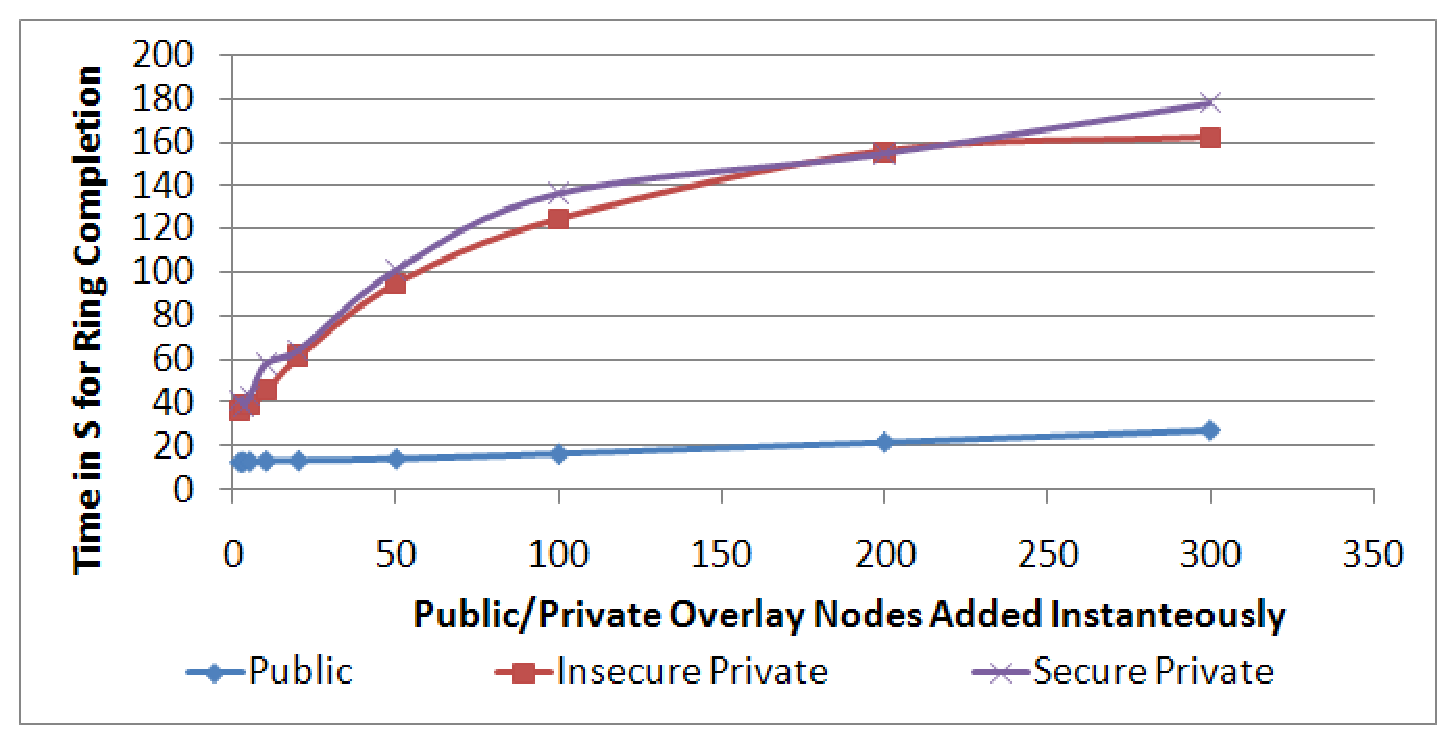
\includegraphics[width=4in]{mass_join.eps}
\caption[Large simultaneous private pool joins.]{The time to form private
overlay using a public overlay with 200 nodes after simultaneously turning on
various counts of private overlay nodes.}
\label{fig:big_join}
\end{figure}

\begin{figure}[ht]
\centering
\includegraphics[width=4in]{bandwidth.eps}
\caption[Bandwidth comparison of insecure and secure overlays.]{Bandwidth used
in a systems with and without security during steady state operations
consisting of 200 public nodes and various sized paired public / private nodes.
Those lines labeled ``static'' have DHT lists queried every 5 minutes whereas
in ``dynamic'' queries are made using an exponential back-off policy starting
at 30 seconds up to a maximum of 60 minutes.  Bandwidth is in bytes / second, a
negligible amount of bandwidth for DSL and Cable Internet.}
\label{fig:vpo_bandwidth}
\end{figure}

\begin{figure}[ht]
\centering
\includegraphics[width=4in]{revocation_sim.eps}
\caption[Simulated broadcast revocation evaluation.]{The time delay and
bandwidth used during the time between revoking a node and notifying nodes of
the revocation using simulations.  (Broadcast has been abbreviated to
``Bcast'').}
\label{fig:revocation_sim}
\end{figure}

\begin{figure}[ht]
\centering
\includegraphics[width=4in]{revocation_mod.eps}
\caption[Modeled broadcast revocation evaluation.]{The time delay and bytes
transferred during the time between revoking a node and notifying nodes of the
revocation using the modeler.  (Broadcast has been abbreviated to ``Bcast'').}
\label{fig:revocation_mod}
\end{figure}

